\section{Research Design} 
\label{sec:research-design}

This sample research-design section shows where authors can describe the data, measurement, and estimation procedures. Authors can first identify the unit of analysis, sampling frame, and period covered by the study. Another sentence can define the principal variables and explain how each measure corresponds to the theoretical concepts. A subsequent sentence can summarize the estimation strategy and the treatment of uncertainty. This sample sentence demonstrates a textual citation to \citet{Imai2011}. Figure~\ref{fig:sampleflowchart} provides a generic example of a research workflow.\begin{figure}[!t]
  \centering

  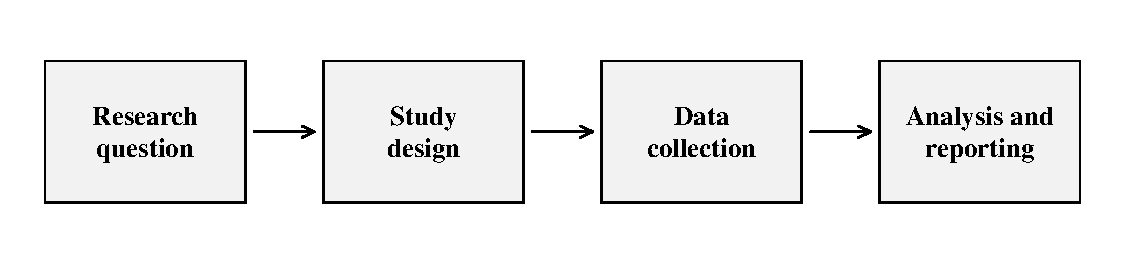
\includegraphics[width=\textwidth]{figures/sample_flowchart.pdf}

  \begin{spacing}{1.25}
    \caption{Sample Research Workflow. \textit{Note: The flowchart presents four generic stages that authors can adapt to their research design.}}
    \label{fig:sampleflowchart}
  \end{spacing}

\end{figure}%
 This sample sentence shows how the paragraph continues after a modular figure input. Replace these sample sentences and the flowchart with material tailored to the study.

\FloatBarrier
